%! Author = Pascal Bakker
%! Date = 04/05/2024

%-------------------------------------------------------------------------------
% TEMPLATE
%-------------------------------------------------------------------------------
\documentclass[balance=false,nonacm,sigconf]{acmart}

\settopmatter{printacmref=false} % Removes citation information below abstract
\renewcommand\footnotetextcopyrightpermission[1]{} % removes footnote with conference information in first column

\AtBeginDocument{%
    \providecommand\BibTeX{{%
        \normalfont B\kern-0.5em{\scshape i\kern-0.25em b}\kern-0.8em\TeX}}}

% support special characters
\usepackage[T1]{fontenc}
\usepackage{lmodern}

%-------------------------------------------------------------------------------
% PACKAGES FOR URL
%-------------------------------------------------------------------------------
\hypersetup{colorlinks, citecolor=blue, filecolor=blue, linkcolor=blue, urlcolor=blue}
\usepackage{xurl}

%-------------------------------------------------------------------------------
% PACKAGES AND COMMANDS FOR TABLES
%-------------------------------------------------------------------------------
\usepackage{longtable}
\usepackage{multirow}
\usepackage{adjustbox}
\usepackage{color,colortbl,xcolor}
\usepackage{array}
\newcommand*{\thead}[1]{\multicolumn{1}{c}{#1}}
\newcommand{\tabitem}{~~\llap{\textbullet}~~}
%\newcolumntype{L}[1]{>{\raggedright\renewcommand{\newline}{\\}\arraybackslash\hspace{0pt}}m{#1}}
%\newcolumntype{C}[1]{>{\centering\renewcommand{\newline}{\\}\arraybackslash\hspace{0pt}}m{#1}}
%\newcolumntype{R}[1]{>{\raggedleft\renewcommand{\newline}{\\}\arraybackslash\hspace{0pt}}m{#1}}


%-------------------------------------------------------------------------------
% PACKAGES FOR FIGURES
%-------------------------------------------------------------------------------
\usepackage{graphicx,graphics,float,subfigure,wrapfig,epstopdf}
\usepackage{dblfloatfix} %to fix the problem of [h!] [t!] [!b]
\epstopdfsetup{update}

%-------------------------------------------------------------------------------
% PACKEGE FOR CREATING GANTT VISUALIZATION (PLANNING TABLE)
%-------------------------------------------------------------------------------
\usepackage{pgfgantt}
\usepackage{datetime2,datetime2-calc}

%-------------------------------------------------------------------------------
% CREATING COMMANDS FOR AUTOREF
%-------------------------------------------------------------------------------
\renewcommand{\chapterautorefname}{\S}
\renewcommand{\sectionautorefname}{\S}
\renewcommand{\subsectionautorefname}{\S}
\renewcommand{\subsubsectionautorefname}{\S}
\newcommand{\subfigureautorefname}{\figureautorefname}

%-------------------------------------------------------------------------------
% COPYRIGHT
%-------------------------------------------------------------------------------
\setcopyright{acmcopyright}
\copyrightyear{2024}
\acmYear{2024}

%-------------------------------------------------------------------------------
% BEGIN DOCUMENT
%-------------------------------------------------------------------------------
\begin{document}

%-------------------------------------------------------------------------------
% TITLE
%-------------------------------------------------------------------------------
    \title[Automating the Cybersecurity Triage Process]{Automating the Cybersecurity Triage Process: A Comparative Study on the Performance of Large Language Models}

%-------------------------------------------------------------------------------
% AUTHORS
%-------------------------------------------------------------------------------
    \author{Pascal Bakker}
    \email{p.n.bakker@student.utwente.nl}
    \affiliation{%
        \institution{University of Twente}
        \streetaddress{P.O. Box 217}
        \city{Enschede}
        \country{The Netherlands}
        \postcode{7500AE}
    }

%-------------------------------------------------------------------------------
% ABSTRACT AND KEYWORDS
%-------------------------------------------------------------------------------
    % context
% problem
% difference from literature
% proposal
% expected contributions
\begin{abstract}
    In Security Information and Event Management, alarms are created when certain conditions are met.
    Security analysts have the task to inspect alarms to filter false positives and identify their severity: triage.
    This process is complicated and time-consuming, limiting the depth and speed of investigations.
    Whereas other proposed optimizations and automations appear to be very promising, rapid advancements in Natural Language Processing and the development of Large Language Models (LLMs) opened up new possibilities to speed up the triage process.
    This research will identify ways in which LLMs can optimize triage, evaluate the performance of these techniques and offer a comparison between different LLMs.
    The results of this research are expected to help security teams in making informed implementation decisions when optimizing the triage process.
\end{abstract}
    \keywords{%
        Cybersecurity,
        triage,
        analysis,
        large language model,
        natural language processing,
        automation
    }

%-------------------------------------------------------------------------------
%-------------------------------------------------------------------------------
    \maketitle

%-------------------------------------------------------------------------------
% SECTIONS
%-------------------------------------------------------------------------------
    \section{Introduction} 
\label{sec:introduction}


\comment{The Introduction section has more or less the same structure as your abstract. The difference is that in the abstract each part is one statement/phrase, while in the introduction each part is a paragraph. So, (i) context, (ii) problem, (iii) proposal, and your most astonishing (iv) finding. Of course in the Introduction section you can give far more details than in the abstract. Avoid to copy and paste statements, re-write with different words.}

\comment{In addition to the structure that you already know you should include your \textit{research questions} between the ``proposal'' paragraph and the ``findings''. The statement that precede the RQ is something like the following: }

To pursue our goal, we have defined the following research questions (RQ) as the basis of our research: 
\begin{itemize}	
	\item \textbf{RQ1:} What are ..?
	\item \textbf{RQ2:} How to ... ?
	 \item \textbf{RQ3:} How to ...?
\end{itemize}



\comment{Please, avoid "yes or no" questions. Make questions that your reader are not able to answer immediately. Usually the questions depend on each other, it means that to answer one question you must answer the one before.}

\comment{Before a little bit of your most astonishing findings you must to introduce the structure of your paper (or proposal). Usually the text looks like the following.}
 
``The remainder of this paper (or proposal) is organized as follows. Section 2 will discuss the approaches expected for answering each research question. After that, we present a preliminary planning for the research questions in Section 3. Finally, we conclude with a proposal and planning for the thesis structure in Section 4.'' 






    \section{Related Work}
\label{sec:related-work}

*Check connectedpapers.com

\begin{enumerate}
    \item A Survey of Large Language Models in Cybersecurity
    \item Review of Generative AI Methods in Cybersecurity
    \item
\end{enumerate}

For the phase after the proposal you should re-read those interesting papers and take note of their "related work" papers. Read those papers and update the Excel Sheet.

\textbf{NOTE: that the final goal of this section is a table that summarizes the characteristics of each paper and your critical analysis to highlight the existing gaps of research.}

Examples of how to make a reference:
\begin{itemize}
    \item $\backslash$citep outputs:~\citep{jjsantanna2015IM1}
    \item $\backslash$citet outputs: \citet{jjsantanna2015IM1}
\end{itemize}

    \section{Methodologies}
<brief summary explaining the content and the connection><you could even to make a picture explaining how the parts connect for example a conceptual figure with your idea (if possible). On this, I must say that Figures MUST be in pdf format (I like to use Inkscape to create my figures, then I export to pdf) [ask me how, for help]> 

\subsection{On answering RQ1}

\subsection{On answering RQ2}

\subsection{On answering RQ3}
\begin{figure}[h!]
	\label{fig:approach}
	\centering
	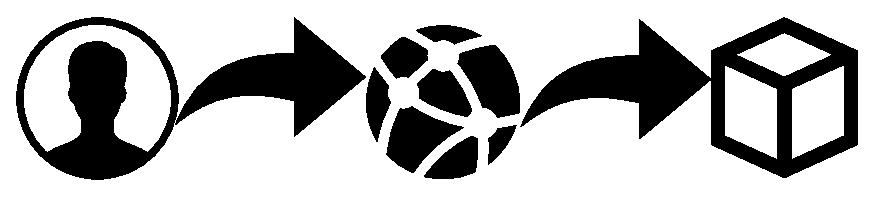
\includegraphics[width=0.45\textwidth]{figs/example.eps}
	\caption{Example of Figure.}
\end{figure}
    \section{Expected Results}
\label{sec:expected-results}

After answering the research questions, it is expected that the proposed techniques significantly reduce the time that
security analysts need when triaging the three tested types of security alarms, as well as reducing the chances of
human error.

Additionally, the study will determine suitable metrics to evaluate LLMs in the context of incident response.
The findings of this research will also provide useful insights that can be reapplied in the contexts of other
alarm types, leading to an increase in coverage of LLMs in the triage process.

Lastly, the comparisons of the different models should allow security teams and organizations to make informed decisions
about which models are the most effective to implement into the incident response workflow.
    \section{Planning}
\label{sec:planning}

This section discusses the proposed planning of the study which will act as a guideline throughout the research process.
Besides this proposal, the planning separates the study into the categories `research`, `paper` and `presentation`,
as is shown in the Gantt chart in Figure\ \ref{fig:gantt-chart}.

Of the three research questions, most time is allocated to research question one, because it involves a literature
review, full understanding of the triage process and an implementation of the automation.
Submission deadlines are shown as diamonds with white indicating draft submissions and black indicating final
submissions.
These deadlines consist of the following:

\begin{itemize}
    \item May 9th: Research proposal draft
    \item May 13th: Research proposal acceptance
    \item June 23rd: Draft paper submission
    \item June 30th: Final paper submission
    \item July 4th: Camera ready paper submission
    \item July 5th: Conference presentation
\end{itemize}

%-------------------------------------------------------------------------------
% GANTT CHART
%-------------------------------------------------------------------------------

\definecolor{proposal}{RGB}{252,106,148} % dark pink
\definecolor{research}{RGB}{85,159,237} % blue
\definecolor{writing}{RGB}{237,189,85} % orange-yellow
\definecolor{presentation}{RGB}{74,217,121} % green
\definecolor{draft}{RGB}{255,255,255} % white
\definecolor{final}{RGB}{0,0,0} % black

\setganttlinklabel{f-s}{} % disable "finish-to-start" label

% ensure vgrid starts at first day of week
\DTMcomputedayofweekindex{2024-05-01}{\startdow}
\newcount\off\off\startdow\multiply\off -1\advance\off 6
\ifnum\off=0
    \ganttset{vgrid={dotted, *{\the\off}{draw=none}}}
\else
    \if\startdow=0
        \ganttset{vgrid={*{\startdow}{draw=none}, dotted}}
    \else
        \ganttset{vgrid={*{\the\off}{draw=none}, dotted, *{\startdow}{draw=none}}}
    \fi
\fi

\begin{figure}[H]
    \begin{center}
        \scalebox{0.85}{
            \begin{ganttchart}
                [
                time slot format=isodate,
                time slot unit=day,
                calendar week text={\currentweek},
                y unit title=0.4cm,
                y unit chart=0.6cm,
                x unit=0.1cm,
                title label anchor/.style={below=-1.6ex},
                title height=1,
                progress label text={},
                group height=0.2,
                group top shift=0.4,
                group left shift=-0.25,
                group right shift=0.25,
                group/.append style={fill=gray},
                bar height=0.5,
                bar top shift=0.25,
                milestone left shift=-0.25,
                milestone right shift=1.25,
                link type=f-s
                link/.style={->},
                ]{2024-05-01}{2024-07-5}
                %labels
                \gantttitlecalendar{year, month=name, week} \\
                %
                \ganttbar[bar/.append style={fill=proposal}]{Research Proposal}{2024-05-01}{2024-05-9}\\
                \ganttmilestone[milestone/.append style={fill=draft}]{Submissions}{2024-05-09}
                \ganttmilestone[milestone/.append style={fill=final}]{}{2024-05-13} \\\\
                %
                \ganttgroup{Research}{2024-05-14}{2024-06-24}\\
                \ganttbar[bar/.append style={fill=research}]{RQ1}{2024-05-14}{2024-06-07}\\
                \ganttlinkedbar[bar/.append style={fill=research}]{RQ2}{2024-06-10}{2024-06-17}\\
                \ganttlinkedbar[bar/.append style={fill=research}]{RQ3}{2024-06-20}{2024-06-24}\\\\
                %
                \ganttgroup{Paper}{2024-05-14}{2024-06-30}\\
                \ganttbar[bar/.append style={fill=writing}]{Writing}{2024-05-14}{2024-06-30}\\
                \ganttmilestone[milestone/.append style={fill=draft}]{Submissions}{2024-06-23}
                \ganttmilestone[milestone/.append style={fill=final}]{}{2024-06-30}
                \ganttmilestone[milestone/.append style={fill=final}]{}{2024-07-04}\\\\
                %
                \ganttgroup{Presentation}{2024-06-22}{2024-07-05} \\
                \ganttbar[bar/.append style={fill=presentation}]{Preparation}{2024-06-22}{2024-07-05} \\
                \ganttmilestone[milestone/.append style={fill=final}]{Conference}{2024-07-05}
            \end{ganttchart}
        }
    \end{center}
    \caption{Gantt chart of proposed planning}
    \label{fig:gantt-chart}
\end{figure}
    \section{Use of AI}
\label{sec:use-of-ai}

Besides the use of LLMs as needed for this research, during the preparation of this work, the author(s) will use
generative AI tools such as ChatGPT, LLama3, Grammarly, and JetBrains Grazie and full line code completion for the
following purposes:

\begin{itemize}
    \item Find definitions of terms and concepts when conventional tools and search engines are unsatisfactory.
    \item Check and correct the spelling of words and grammar of sentences.
    \item Improve the readability of sentences and paragraphs through rewording and restructuring.
    \item Use code completion functionality to speed up programming tasks.
\end{itemize}

After using these tools/services, the author(s) will review and edit the content as needed and take full
responsibility for the content of the work.
The services will not be used to produce scientific insights, create figures, draw conclusions or provide
recommendations.

%-------------------------------------------------------------------------------
% REFERENCES
%-------------------------------------------------------------------------------
    \bibliographystyle{ACM-Reference-Format}
    \bibliography{bibliography}

%-------------------------------------------------------------------------------
% END DOCUMENT
%-------------------------------------------------------------------------------
\end{document}
\endinput
